\documentclass[paper-main.tex]{subfiles}

\begin{document}

\begin{figure}
	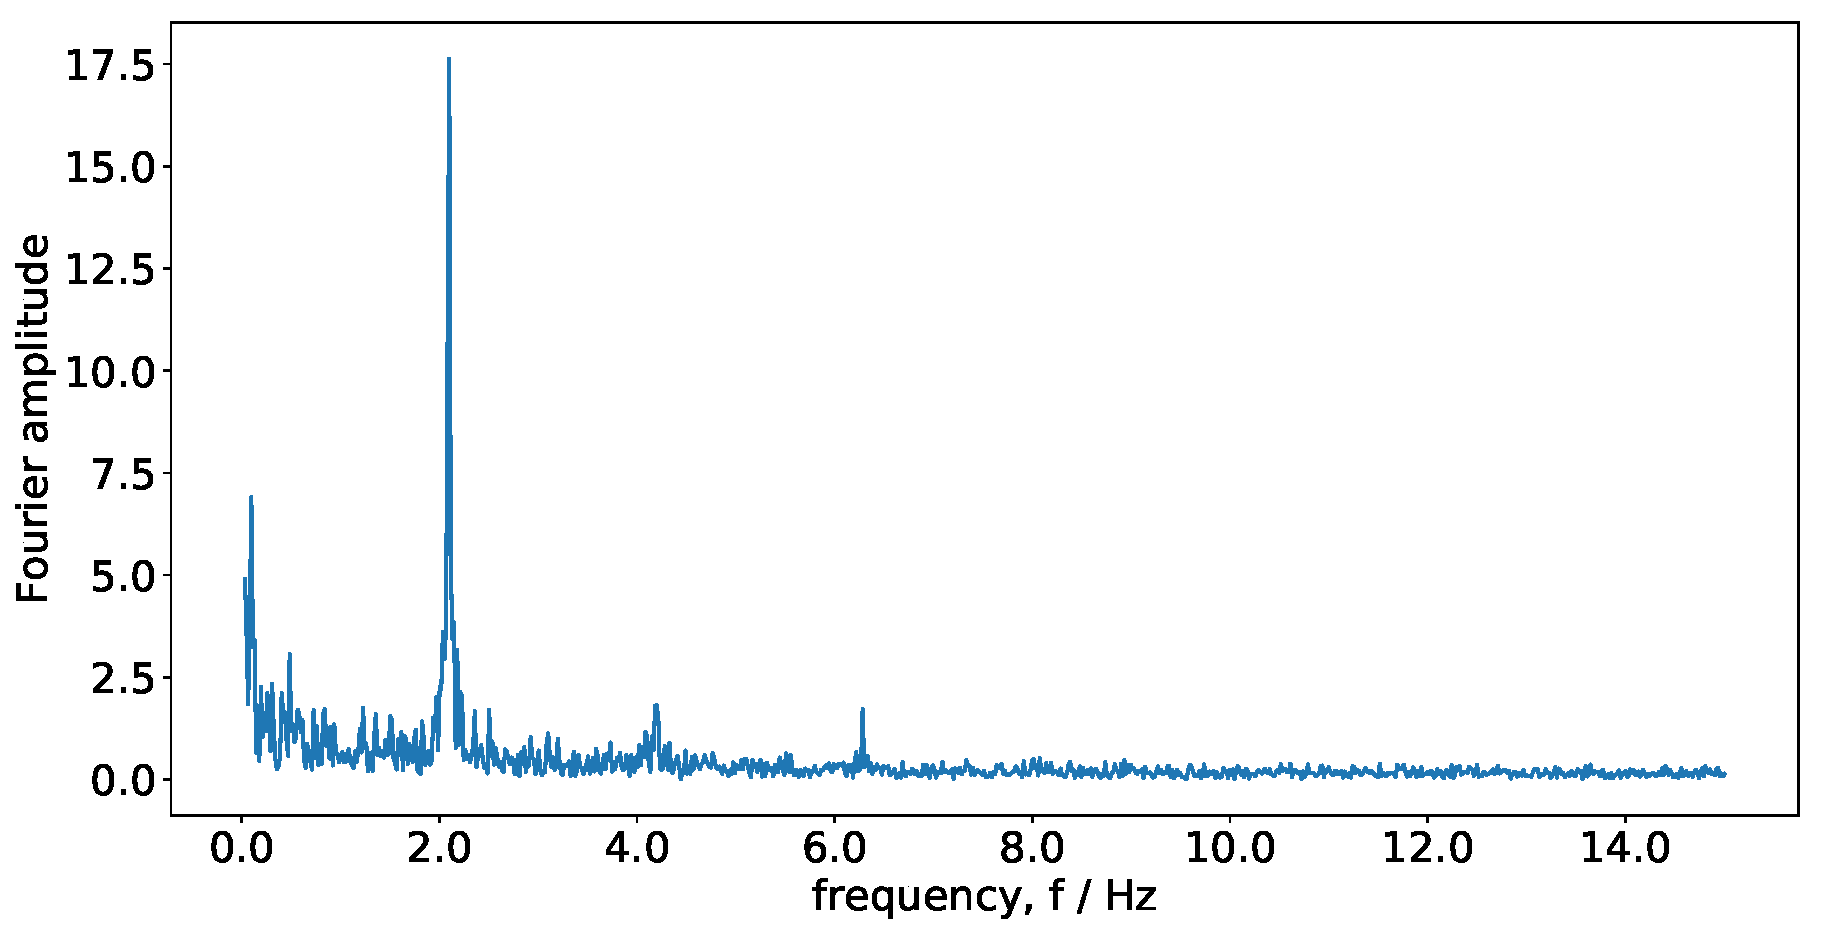
\includegraphics[width=.49\textwidth]{figures/webcam_expt_4_0209-cropped.pdf}
	\caption{\label{fig:webcam_spectrum}
Recovery of a tone at a constant frequency: Here we plot the Fourier amplitude of the intensity pattern against frequency.
The injected signal has a frequency of $2.09\,{\rm Hz}$, while the recovered signal peaks at $2.099\,{\rm Hz}$ and has a FWHM of $0.033\,{\rm Hz}$.
The plot also shows two harmonics at $4.19\,{\rm Hz}$ and $6.28\,{\rm Hz}$ with normalised amplitude to the primary peak of $0.103$ and $0.098$ respectively.
}	
\end{figure}


Continuous-wave searches look for nearly monochromatic signals. In this section we consider a simple sinusoidal tone; a signal at a single constant frequency.

As described in Section~\ref{sec:ifo}, the audio signal is played through a speaker fixed to the back of M2. The intensity of the interference pattern is measured at a single point on the screen using a commercial USB webcam (see Fig.~\ref{fig:ifo_schematic_webcam}). The webcam samples at a rate of $30\,{\rm Hz}$, which limits the spectral content of observable signals to below $15\,{\rm Hz}$, the Nyquist frequency. A tone with a frequency of 2.09Hz is played through the speaker for one minute and the interference pattern is recorded by the webcam.


We take data from an off-centre pixel as indicated by the pink star in Fig.~\ref{fig:interference_pattern}. The pixel intensity in the green-channel of the video (the webcam records in three colour channels: red, blue, and green) is used to approximate the total intensity of the interference pattern. This is because the laser emits monochromatic green light at $532\,{\rm nm}$.
The amplitude of the Fourier transform of the recorded signal is shown in Fig.~\ref{fig:webcam_spectrum}. We measured a strong signal at $2.099\,{\rm Hz}$ with a full width half maximum (FWHM) of $0.033\,{\rm Hz}$. Although this range doesn't contain our injected frequency, the error is not substantial and cannot be heard by the (untrained) human ear.
Two harmonics can also be seen at integer multiples of the peak frequency. The peaks at $4.19\,{\rm Hz}$ and $6.28\,{\rm Hz}$ have amplitudes of $0.103$ and $0.098$ as a fraction of the height of the main peak, respectively. They are likely due to the nonlinear response of the system discussed in Section~\ref{sec:ifo} and Appendix~\ref{app:intensity_derivation}.


In the following section, we use a hidden Markov model technique, commonly used in continuous wave searches, to recover a slowly wandering frequency signal.


\end{document}
